\documentclass{beamer}

\usepackage{graphicx}

\begin{document}
\begin{frame}
\begin{figure}
\centering
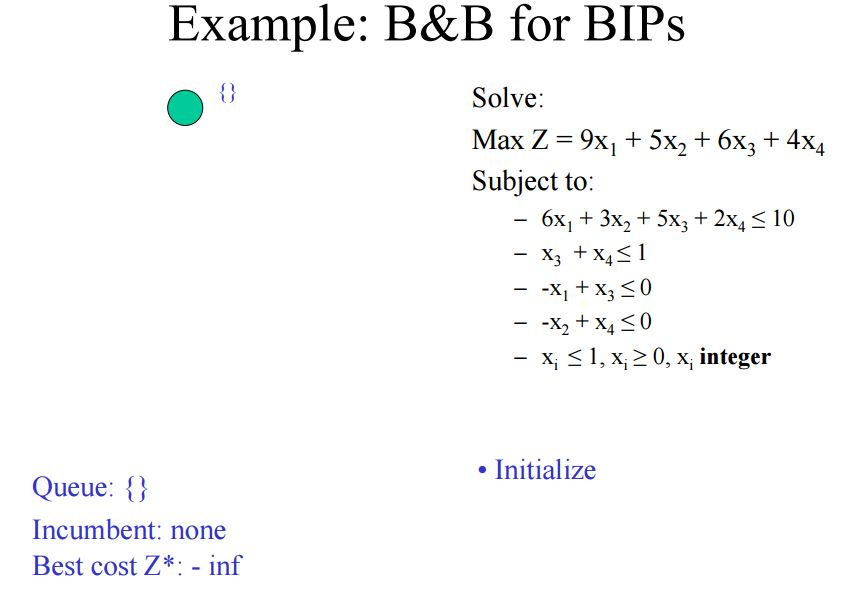
\includegraphics[width=1.1\linewidth]{BB-BIP/BB-BIP1}
\end{figure}
\end{frame}
\begin{frame}
	\begin{figure}
		\centering
		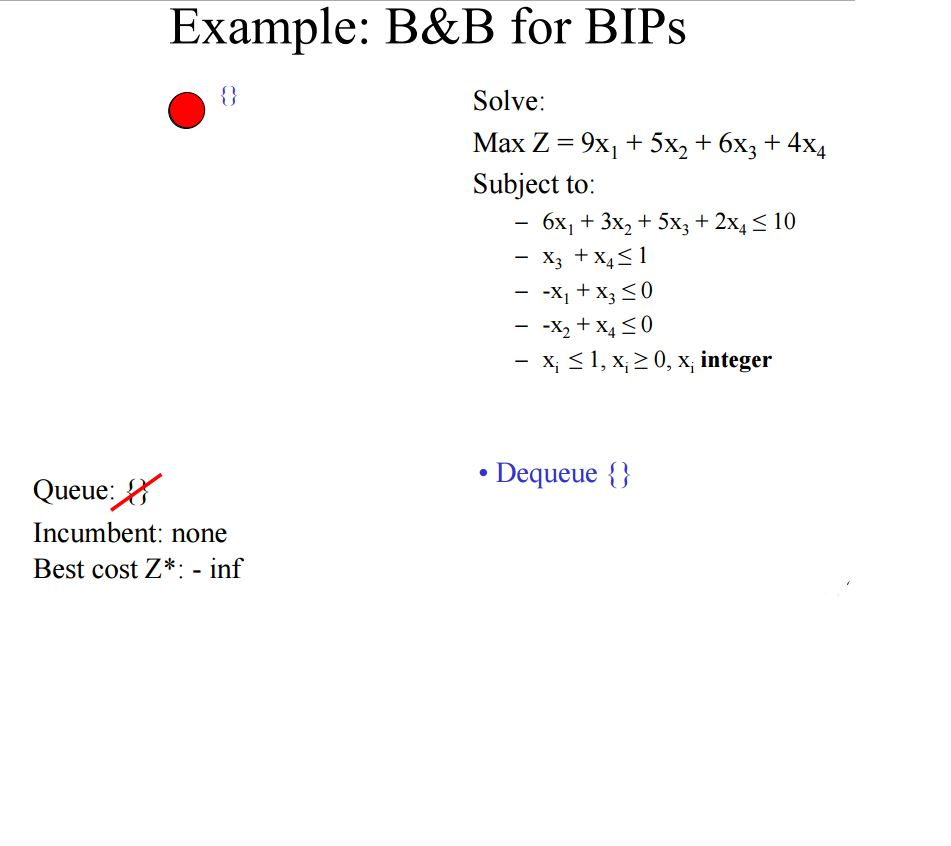
\includegraphics[width=1.1\linewidth]{BB-BIP/BB-BIP2}
	\end{figure}
\end{frame}
\begin{frame}
	\begin{figure}
		\centering
		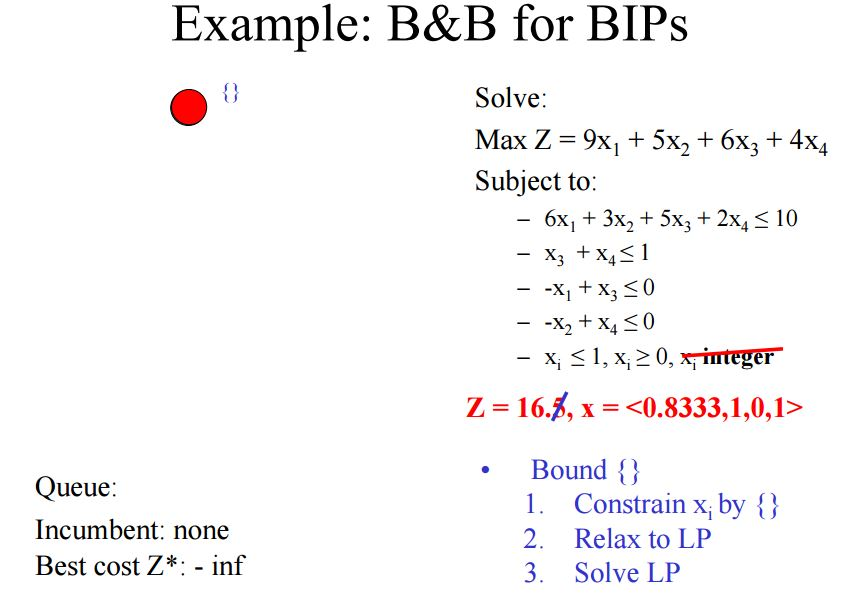
\includegraphics[width=1.0\linewidth]{BB-BIP/BB-BIP3}
	\end{figure}
\end{frame}
\begin{frame}
	\begin{figure}
		\centering
		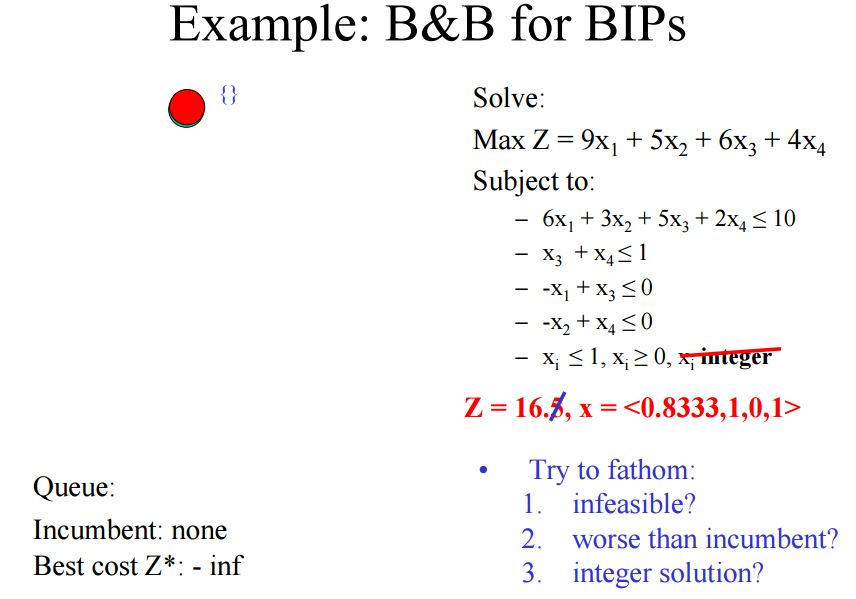
\includegraphics[width=1.0\linewidth]{BB-BIP/BB-BIP4}
	\end{figure}
\end{frame}
\end{document}
